\documentclass[12pt,a4paper]{article}
\usepackage[utf8]{inputenc}
\usepackage[spanish]{babel}
\usepackage{amsmath}
\usepackage{amsfonts}
\usepackage{amssymb}
\usepackage{graphicx}
\usepackage{kpfonts}
\usepackage[left=2cm,right=2cm,top=2cm,bottom=2cm]{geometry}
\title{EV 1-3 CIRCUITO DE CONTROL DE VOLTAJE Y CORRIENTE CON TIRISTORES

\includegraphics [scale=1]{imagenes/UPZMG.png} 
\author{Giovanni Daniel Ruiz Tinoco\\
Alan Antonio Muñoz Juarez\\
\small Sistemas electrónicos de interfaz\\
  \small Universidad Politécnica de la zona metropolitana de Guadalajara\\
  \small 4-B \\
  \small Ing. Mecatrónica\\
\centering
}
}
\begin{document}
\maketitle
\newpage
\begin{center}
\section {MARCO TEÓRICO}
\end{center}
\subsection{¿Qué es un tiristor?}
\begin{flushleft}
El tiristor es un semiconductor de potencia que se utiliza como interruptor, ya sea para conducir o interrumpir la corriente eléctrica, a este componente se le conoce como de potencia por que se utilizan para manejar grandes cantidades de corriente y voltaje, a comparación de los otros semiconductores que manejan cantidades relativamente bajas. \linebreak

Cuando se habla de tiristores comúnmente se cataloga al tiristor como un SRC (silicon controlled rectifier), pero esto no es del todo correcto ya que este tipo es el más popular y conocido pero no es el único que existe. \linebreak
\end{flushleft}
\begin{center}
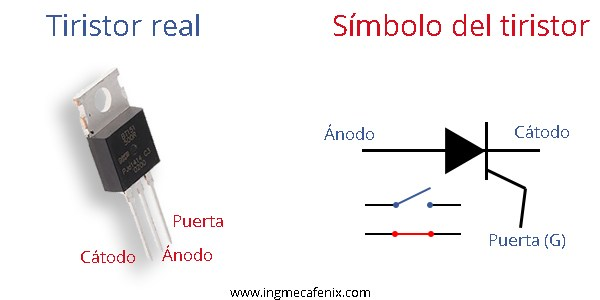
\includegraphics[scale=0.8]{imagenes/tiris.jpg} \linebreak 
\end{center}
\subsection{¿Como funciona un tiristor?}
\begin{flushleft}
Los tiristores están conformados por 3 terminales un ánodo, un cátodo y una compuerta o mejor conocida “gate”, su funcionamiento se asemeja al de un relevador o un interruptor mecánico, Ya que cuando aplicas una corriente a la terminal gate este se activa y obtiene la característica de dejar pasar a la electricidad.
\end{flushleft}
\begin{center}
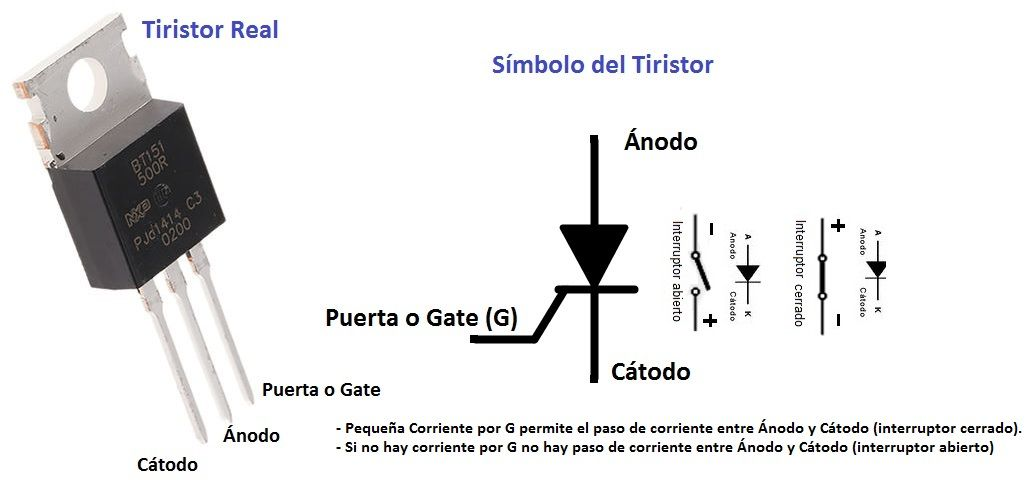
\includegraphics[scale=0.5]{imagenes/tiristor.JPG} 
\end{center}
\subsection{Tipos de tiristores}
\subsubsection{De control de fase o comunicación rápida (SCR)}
\begin{flushleft}
Este tipo es el más común y más utilizado, debido a que son capaces de conmutar rápidamente. Una de las características principales de este tiristor es que solo es capaz de conducir electricidad hacia una sola dirección (como un diodo cuando se polariza directamente), una vez activado este componente no importa si quitas la corriente de la puerta ya que este seguirá activo hasta que se cumpla una de dos condiciones posibles. Para desactivarlo tenemos que cortar el suministro de corriente o llevarla hasta un punto muy bajo que el tiristor sea incapaz de seguir conduciendo.\linebreak
\begin{center}
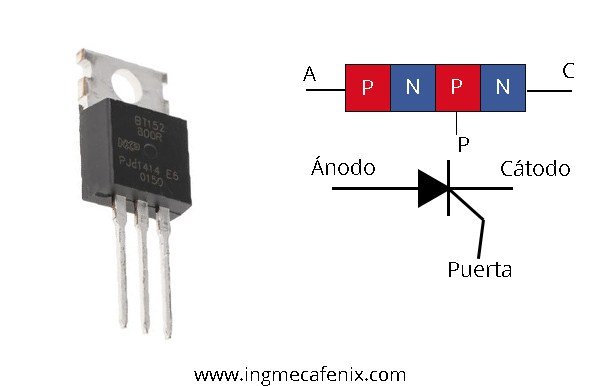
\includegraphics[scale=0.5]{imagenes/scr.JPG} 
\end{center}
\subsubsection{Bidireccionales controlados por face (BCT)}
Este tipo corresponde a dos tiristores en un mismo encapsulado, aun que están juntos no interfieren entre si cada uno tiene sus terminales puerta para ser activados. \linebreak
\begin{center}
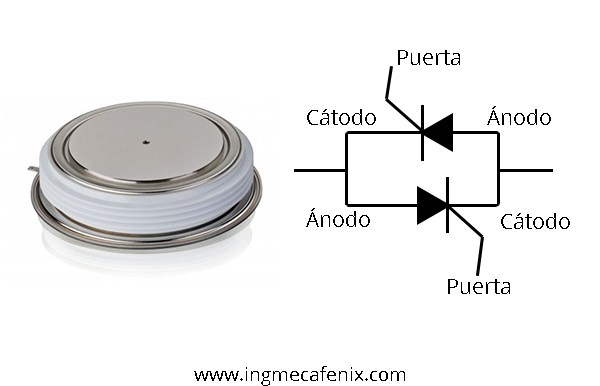
\includegraphics[scale=0.5]{imagenes/btc.JPG} 
\end{center}
\newpage
\subsubsection{Diodo bidireccional (DIAC)}
Aun que este tiene dos terminales y es más parecido a un diodo normal también es considera un tiristor ya que cuando sobre pasa cierto voltaje este se activa, mientras tanto actúa como un interruptor abierto \linebreak
\begin{center}
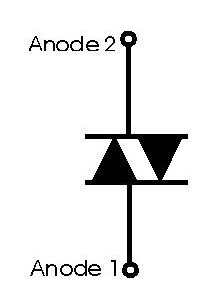
\includegraphics[scale=0.5]{imagenes/diac.JPG} 
\end{center}
\subsubsection{Triodo bidireccional (TRIAC))}
Se usa para la corriente alterna ya que contiene dos tiristores juntos  en un mismo encapsulados, en este ocasión solo cuentan con una terminal puerta y esta es capaz de activar a los dos componentes al mismo tiempo. \linebreak
\begin{center}
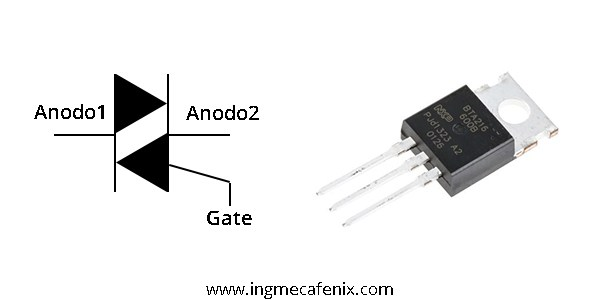
\includegraphics[scale=0.5]{imagenes/triac.JPG} 
\end{center}
\end{flushleft}
\newpage
\begin{center}
\section{Materiales para la práctica}
\end{center}
\begin{flushleft}
-1 Triac\\
-1 Diac\\
-1 foco \\
-1 POT 500k\\
-1 capasitor 400 mf \linebreak
-1 resistencia 1k
Realice la simulación y el circuito del siguiente esquema:\\
\end{flushleft}
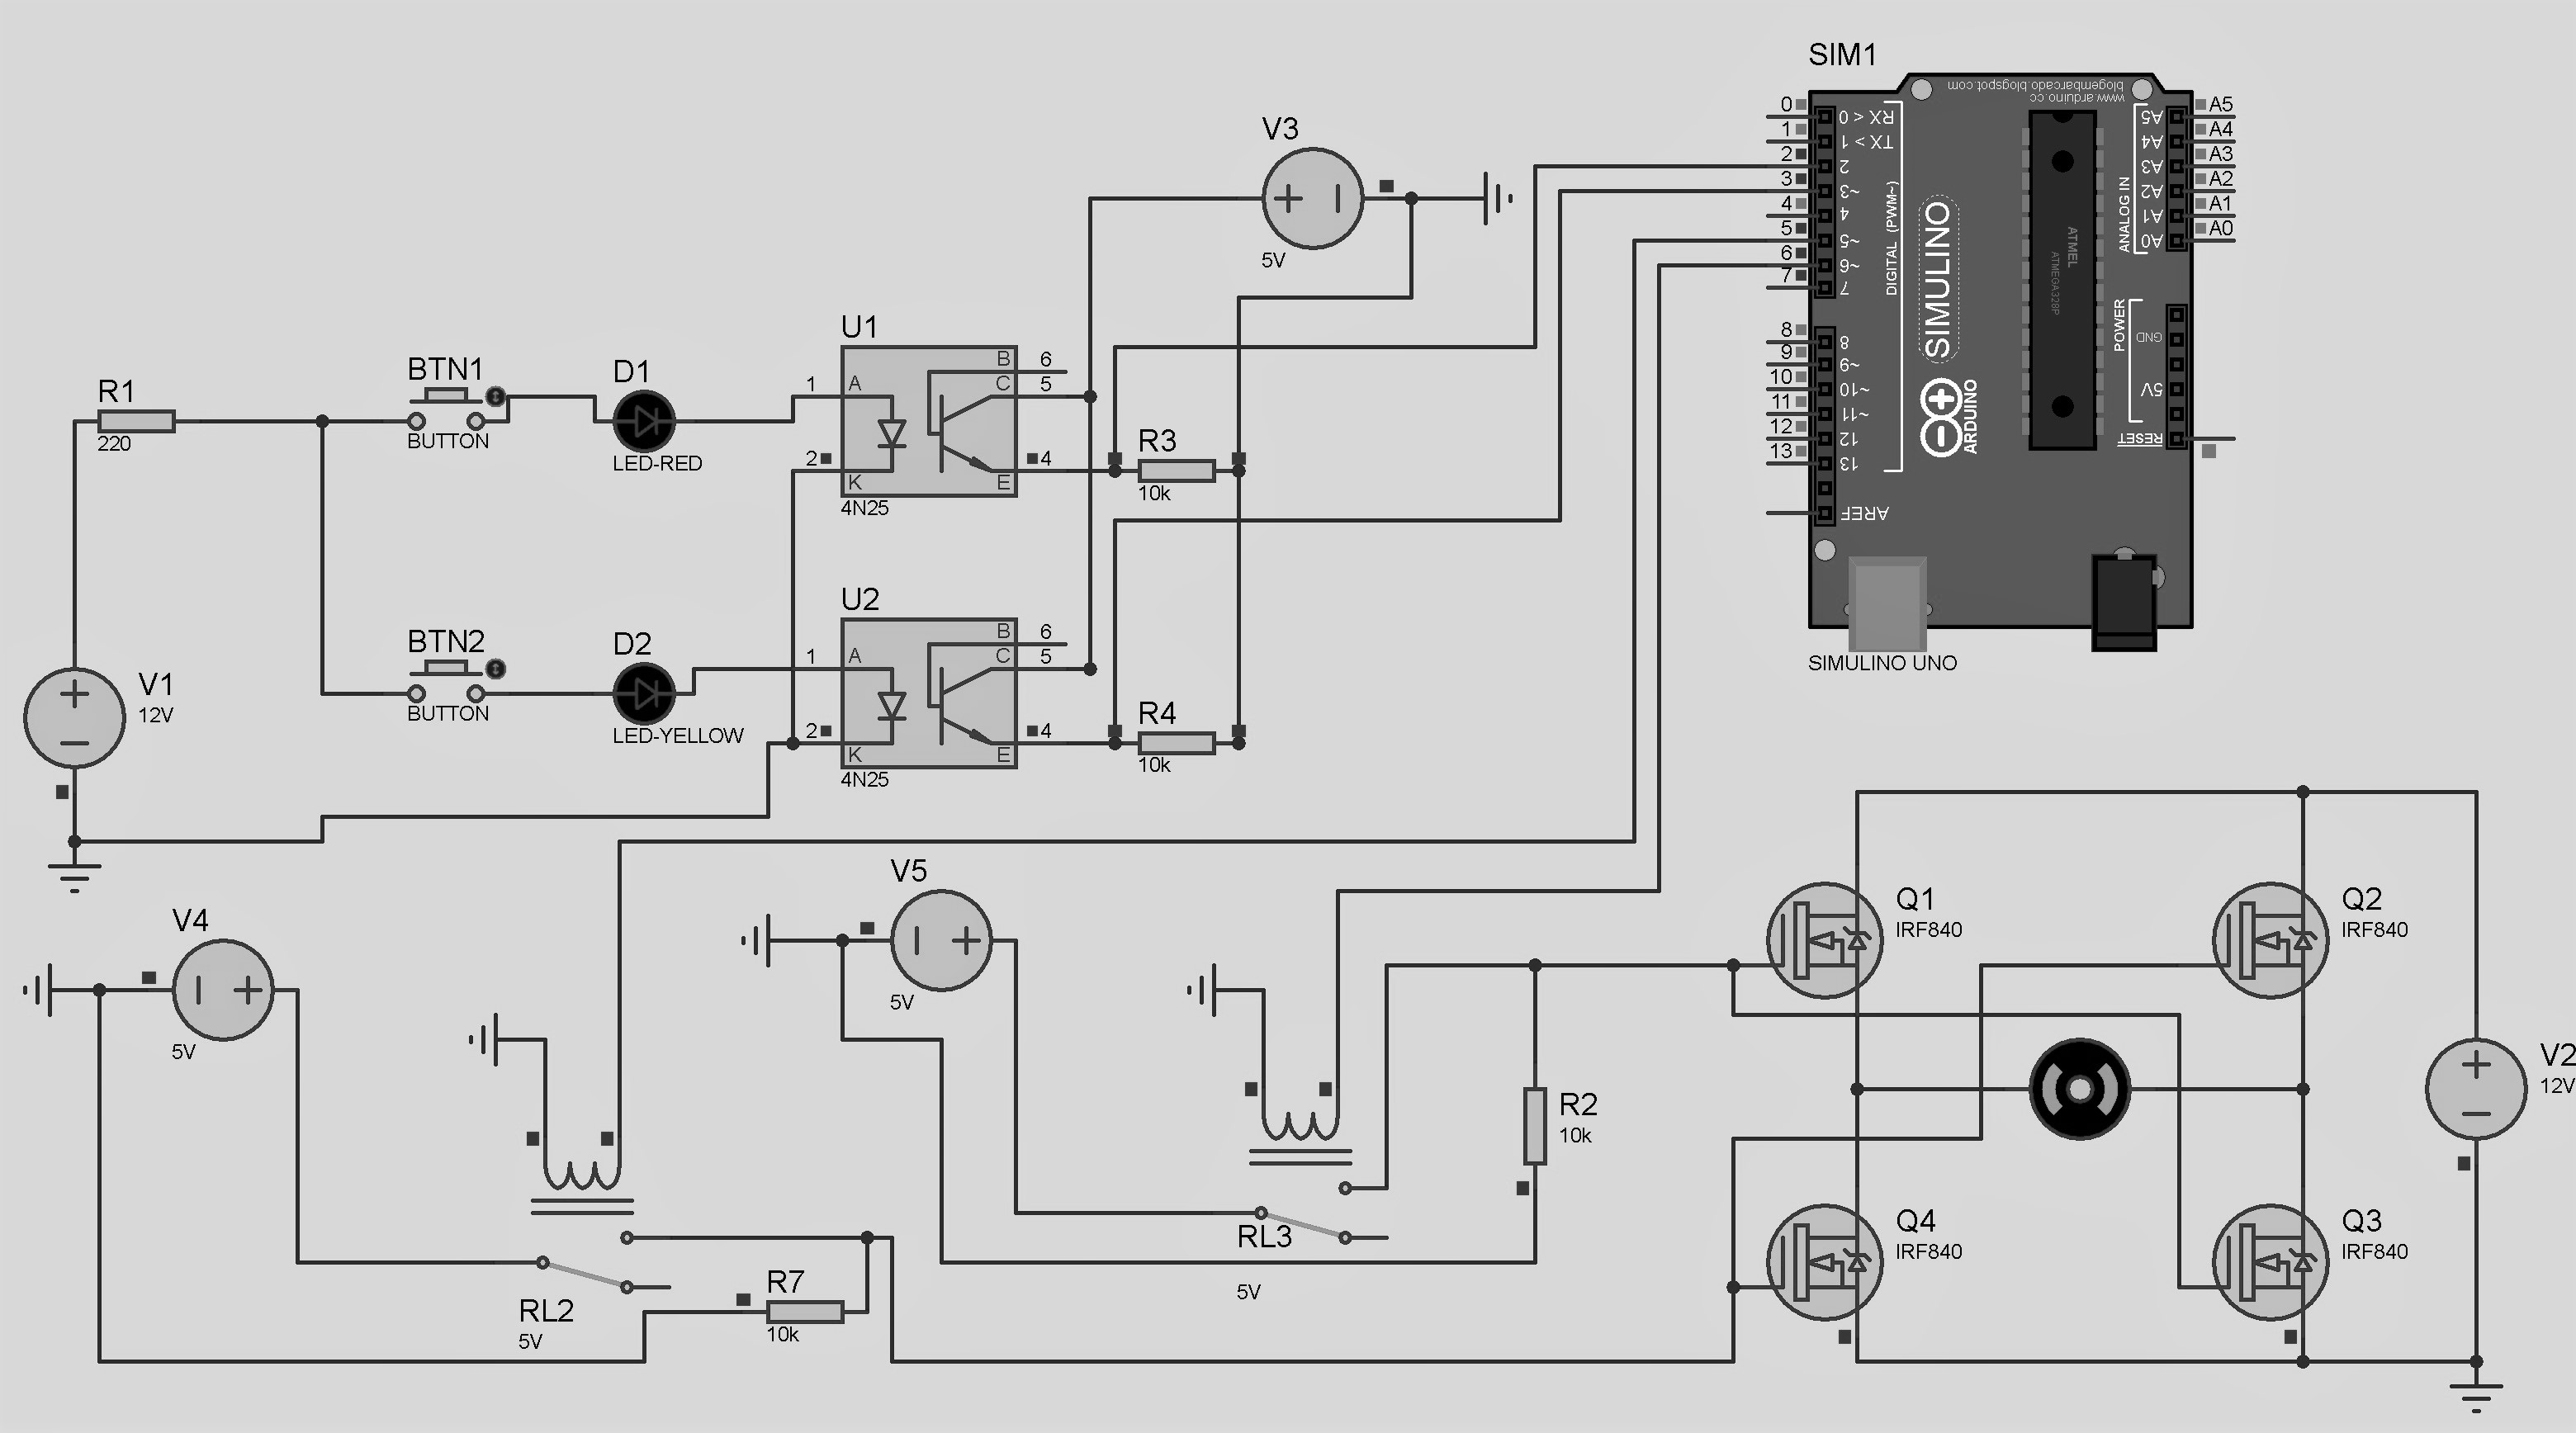
\includegraphics[scale=0.4]{imagenes/circuito.JPG}
\begin{flushleft}
\subsection{Desarrollo de la práctica}
Ahora armaremos el circuito anterior sustituyendo la resistencia 2 por un POT:
\begin{center}
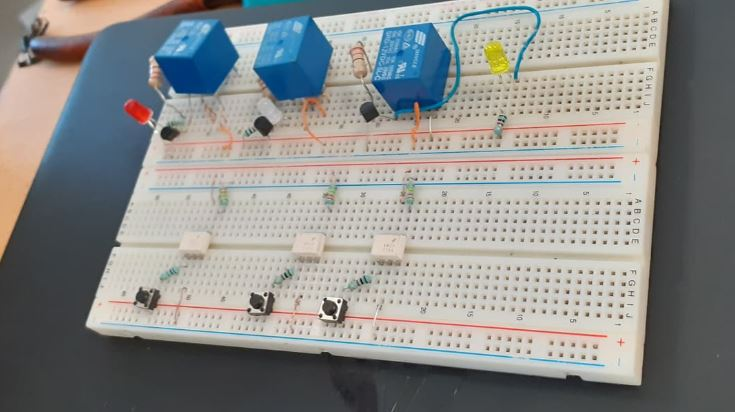
\includegraphics[scale=0.3]{imagenes/circuito1.JPG} \\
\end{center}
\end{flushleft}
\newpage
\subsection{Resultado Final}
\begin{flushleft}
Cuando cambiamos el valor del POT pordemos controlar la intensidad con la que el foco se ilumina, los 4 estados que vamos a menejar son Apagado, intensidad baja, intensidad media e intensidad alta.\linebreak

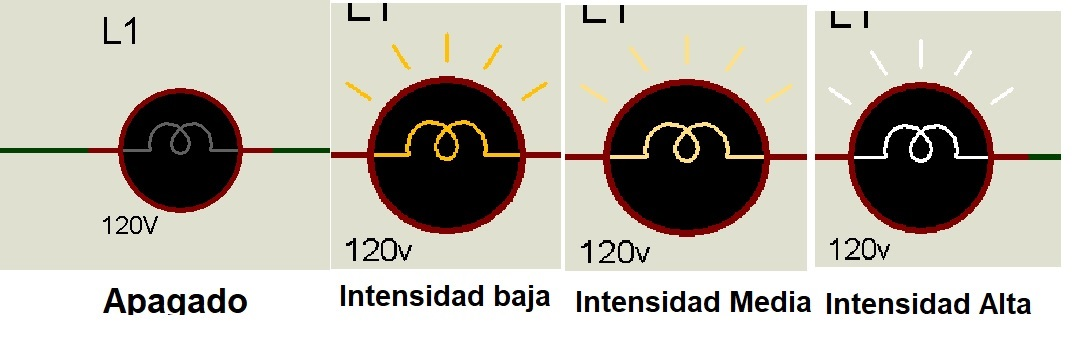
\includegraphics[scale=0.5]{imagenes/Lamp.JPG}
\linebreak
\linebreak
\end{flushleft}
\begin{center}
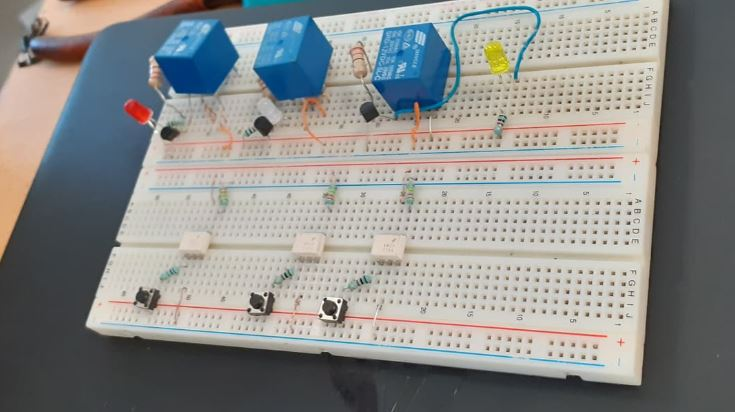
\includegraphics[scale=0.4]{imagenes/circuito1.JPG}
\end{center}
\subsection{Conclusiones}
\begin{flushleft}
En esta practica se aprendió a controlar el disparo de un traic con la ayuda de un capacitor cerámico, esta practica se puede usar para control asistido de diferentes dispositivos los cuales requieran de alimentacion de 120v.
\end{flushleft}
\end{document}

\section{se}